\section{running example}
\begin{frame}[fragile]{running example}
\begin{Verbatim}[fontsize=\small]
$ file mystery
mystery: ELF 64-bit LSB pie executable, x86-64,
version 1 (SYSV), dynamically linked,
interpreter /lib64/ld-linux-x86-64.so.2,
BuildID[sha1]=9819a3cfb39d01ad2a376c54318f104139422a8f,
for GNU/Linux 3.2.0, stripped
\end{Verbatim}
\begin{itemize}
\item LSB = little endian
\item pie = position-independent executable
\item interpreter = program that loads this
\end{itemize}
\end{frame}

\begin{frame}[fragile]{aside: file(1)}
\begin{Verbatim}[fontsize=\small]
$ man file
FILE(1)                      General Commands Manual                    FILE(1)

NAME
       file — determine file type

....
\end{Verbatim}
\hrule
\begin{itemize}
\item looks for ``magic numbers'' near beginning of file data
\item hand-managed database of common patterns
\end{itemize}
\end{frame}

\begin{frame}[fragile]{from file's source}
\begin{Verbatim}[fontsize=\scriptsize]
0   name        elf-le
>16 leshort     0       no file type,
!:mime  application/octet-stream
>16 leshort     1       relocatable,
!:mime  application/x-object
>16 leshort     2       executable,
!:mime  application/x-executable
>16 leshort     3       ${x?pie executable:shared object},

...
0   string      \177ELF     ELF
!:strength *2
>4  byte        0       invalid class
>4  byte        1       32-bit
>4  byte        2       64-bit
>5  byte        0       invalid byte order
>5  byte        1       LSB
>>0 use     elf-le
>5  byte        2       MSB
>>0 use     \^elf-le
>7  byte        0       (SYSV)
\end{Verbatim}
\end{frame}


\section{finding strings}

\begin{frame}[fragile]{finding strings}
\begin{Verbatim}[commandchars=~\{\},fontsize=\fontsize{9}{10}]
$ hexdump -c mystery
00000000  7f 45 4c 46 02 01 01 00  00 00 00 00 00 00 00 00  |.ELF............|
00000010  03 00 3e 00 01 00 00 00  c0 60 00 00 00 00 00 00  |..>......`......|
00000020  40 00 00 00 00 00 00 00  08 5e 03 00 00 00 00 00  |@........^......|
00000030  00 00 00 00 40 00 38 00  0d 00 40 00 1e 00 1d 00  |....@.8...@.....|
~textit{[... many more lines ...]}
00000e60  00 5f 49 54 4d 5f 64 65  72 65 67 69 73 74 65 72  |._ITM_deregister|
00000e70  54 4d 43 6c 6f 6e 65 54  61 62 6c 65 00 5f 5f 67  |TMCloneTable.__g|
00000e80  6d 6f 6e 5f 73 74 61 72  74 5f 5f 00 5f 49 54 4d  |mon_start__._ITM|
00000e90  5f 72 65 67 69 73 74 65  72 54 4d 43 6c 6f 6e 65  |_registerTMClone|
00000ea0  54 61 62 6c 65 00 77 61  64 64 63 68 00 63 6c 65  |Table.waddch.cle|
00000eb0  61 72 6f 6b 00 6e 6f 65  63 68 6f 00 6d 76 70 72  |arok.noecho.mvpr|
~textit{[... many more lines ...]}
\end{Verbatim}
\end{frame}

\begin{frame}{exercise: heuristic?}
    \begin{itemize}
    \item could scan through pages of hexdump for something interesting\ldots
    \vspace{.5cm}
    \item good heuristic for automating this process?
    \end{itemize}
\end{frame}

\begin{frame}[fragile]{strings utility (1)}
\begin{Verbatim}[fontsize=\fontsize{9}{10}]
$ strings mystery
/lib64/ld-linux-x86-64.so.2
*7lT1
A9B*
m8m7
_ITM_deregisterTMCloneTable
__gmon_start__
_ITM_registerTMCloneTable
waddch
clearok
\end{Verbatim}
\vspace{-1em}
\ldots
\begin{Verbatim}[fontsize=\fontsize{9}{10}]
        prints help
        identify object
        left
        down
        right
\end{Verbatim}
\vspace{-1em}
\ldots
\begin{Verbatim}[fontsize=\fontsize{9}{10}]
        save game
        quit
\end{Verbatim}
\end{frame}

\begin{frame}[fragile]{strings utility (2)}
\begin{Verbatim}[fontsize=\fontsize{9}{10}]
$ strings --bytes=40 mystery
character you want help for (* for all):
you feel a wrenching sensation in your gut
your armor appears to be weaker now. Oh my!
you feel a sting in your arm and now feel weaker
Level: %d  Gold: %-5d  Hp: %*d(%*d)  Str: %2d(%d)  Ac: %-2d  Exp: %d/%ld  %s
Ok, if you want to exit that badly, I'll have to allow it
Hello %s, just a moment while I dig the dungeon...
orry, but your terminal window has too few columns.
Sorry, but your terminal window has too few lines.
please specifiy a letter between 'A' and 'Z'
\end{Verbatim}
\ldots
\end{frame}

\begin{frame}{in Ghidra}
\small (after making new project, loading mystery file) \\
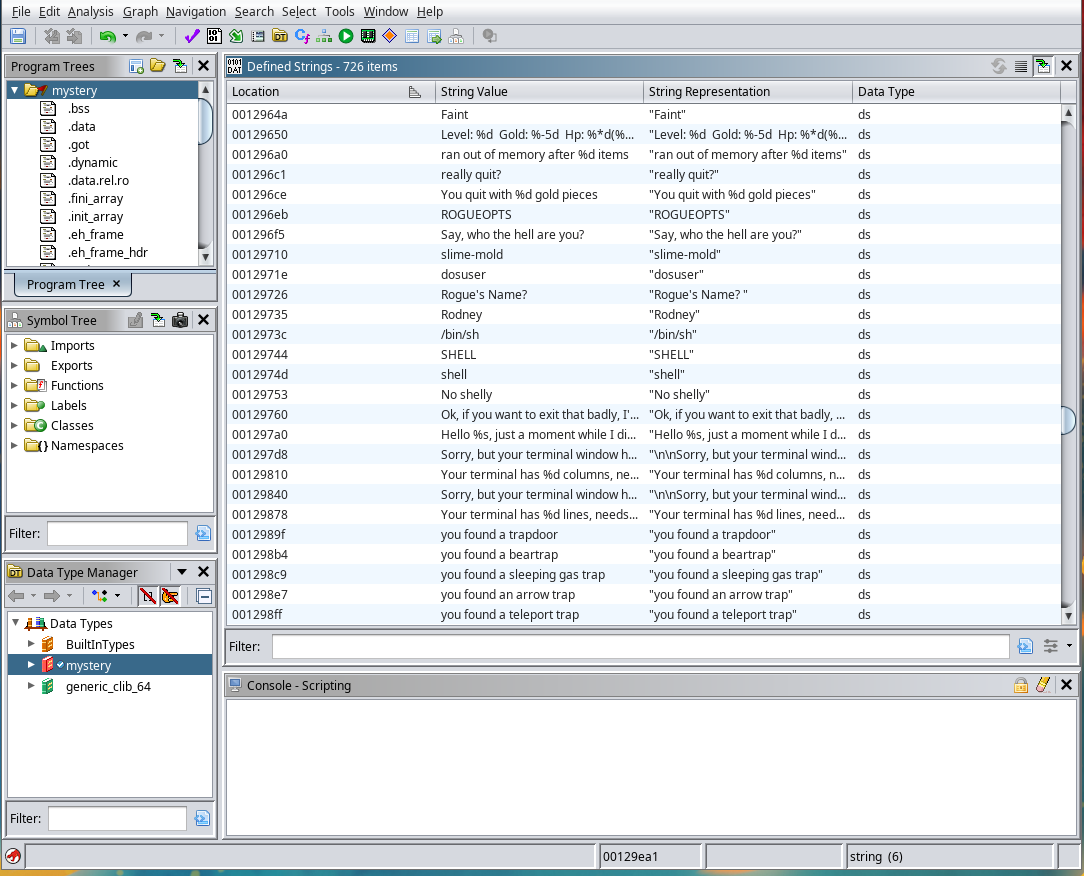
\includegraphics[width=0.8\textwidth]{../re-tools/ghidra-strings-mystery-ex}
\end{frame}



\section{finding library/system calls}

    % FIXME: objdump -R
    % FIXME: objdump -t

\begin{frame}[fragile]{libraries}
\begin{Verbatim}[fontsize=\small]
$ objdump --all-headers mystery
\end{Verbatim}
\ldots
\begin{Verbatim}[fontsize=\small]
Dynamic Section:
  NEEDED               libncurses.so.6
  NEEDED               libtinfo.so.6
  NEEDED               libc.so.6
\end{Verbatim}
\ldots
\end{frame}

\begin{frame}[fragile]{ncurses?}
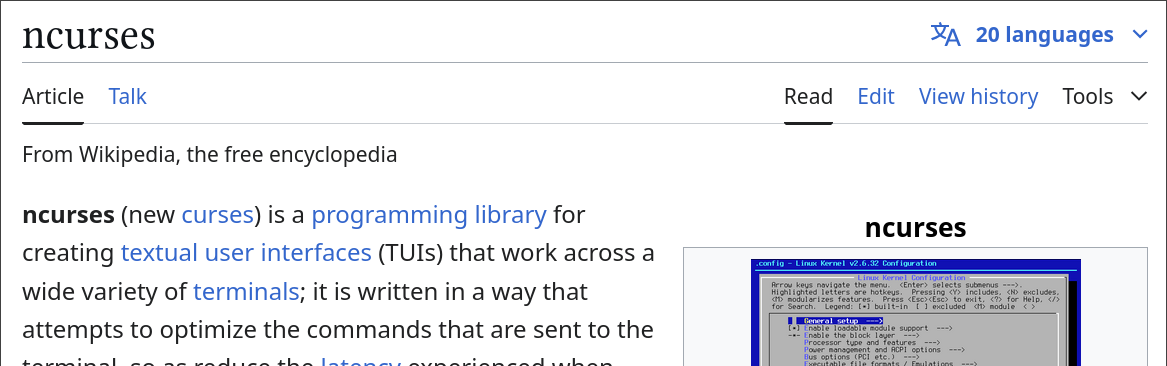
\includegraphics[width=\textwidth]{../re-tools/ncurses-wiki}
\end{frame}

\begin{frame}[fragile]{tinfo? (1)}
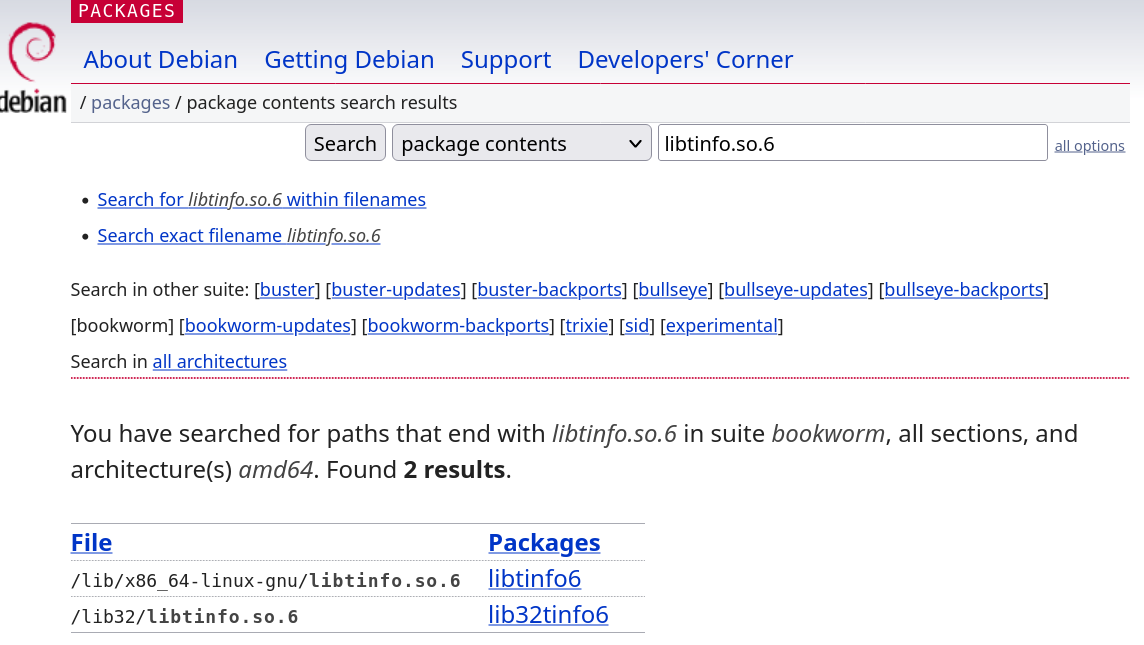
\includegraphics[width=0.7\textwidth]{../re-tools/deb-tinfo1}
\end{frame}

\begin{frame}[fragile]{tinfo? (2)}
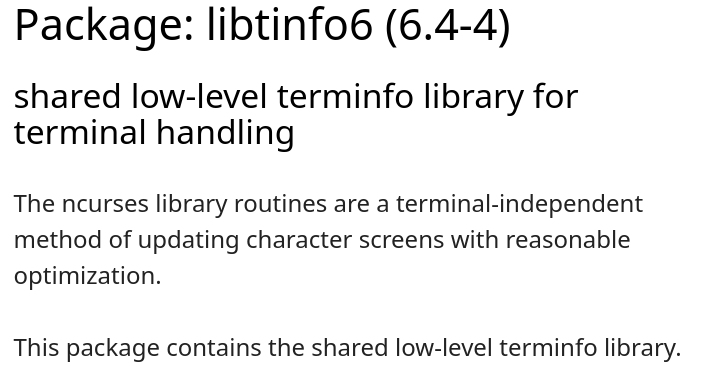
\includegraphics[width=0.7\textwidth]{../re-tools/deb-tinfo2}
\end{frame}

\begin{frame}[fragile]{library calls}
\begin{Verbatim}[fontsize=\fontsize{8}{9}]
$ objdump --dynamic-syms mystery

mystery:     file format elf64-x86-64

DYNAMIC SYMBOL TABLE:
0000000000000000      DF *UND*  0000000000000000 (GLIBC_2.3)  __ctype_toupper_loc
0000000000000000      DF *UND*  0000000000000000 (GLIBC_2.2.5) getenv
0000000000000000      DF *UND*  0000000000000000 (NCURSES6_5.0.19991023) wattrset
0000000000000000      DF *UND*  0000000000000000 (GLIBC_2.2.5) free
0000000000000000      DF *UND*  0000000000000000 (NCURSES6_TINFO_5.0.19991023) flushinp
0000000000000000      DF *UND*  0000000000000000 (GLIBC_2.2.5) localtime
0000000000000000      DF *UND*  0000000000000000 (GLIBC_2.34) __libc_start_main
\end{Verbatim}
\ldots
\begin{Verbatim}[fontsize=\fontsize{9}{10}]
0000000000000000      DF *UND*  0000000000000000 (GLIBC_2.2.5) setuid
\end{Verbatim}
\ldots
\end{frame}

\begin{frame}[fragile]{library calls (Ghidra)}
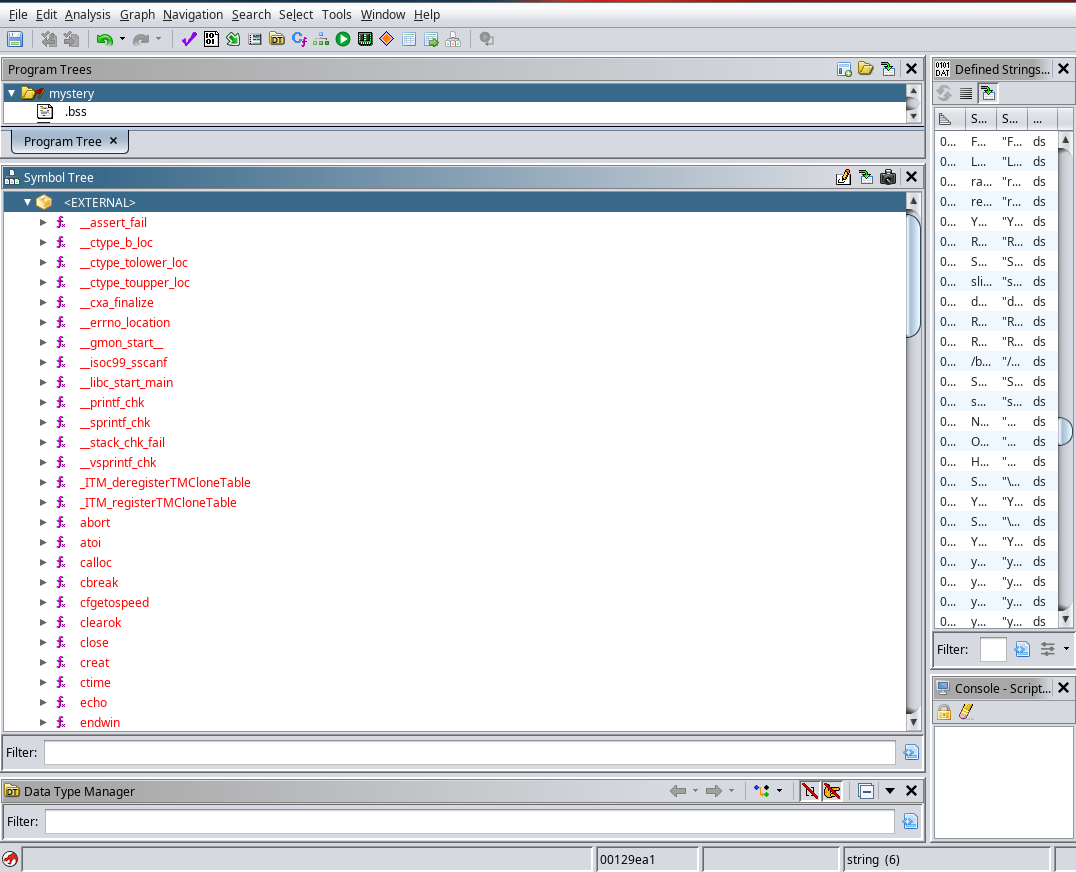
\includegraphics[width=\textwidth]{../re-tools/ghidra-mystery-ext}
\end{frame}

\begin{frame}[fragile]{finding library call uses}
{\small {\tt objdump --disassemble --dyanmic-reloc:}}
\begin{Verbatim}[fontsize=\fontsize{9}{10}]
0000000000005b00 <setuid@plt>:
    5b00:▶      f3 0f 1e fa          ▶  endbr64␣
    5b04:▶      f2 ff 25 fd d3 02 00 ▶  bnd jmp *0x2d3fd(%rip) 
			# 32f08 <setuid@GLIBC_2.2.5>
    5b0b:▶      0f 1f 44 00 00       ▶  nopl   0x0(%rax,%rax,1)
\end{Verbatim}
\ldots
\begin{Verbatim}[fontsize=\fontsize{9}{10}]
   2764f:▶      e8 ec e3 fd ff       ▶  call   5a40 <open@plt>
   27654:▶      89 05 fe 48 01 00    ▶  mov    %eax,0x148fe(%rip)        # 3bf58 <LINES@NCURSES6_TINFO_5.0.19991023+0x5244>
   2765a:▶      31 c0                ▶  xor    %eax,%eax
   2765c:▶      e8 2f e1 fd ff       ▶  call   5790 <getuid@plt>
   27661:▶      89 c7                ▶  mov    %eax,%edi
   27663:▶      31 c0                ▶  xor    %eax,%eax
   27665:▶      e8 96 e4 fd ff       ▶  call   5b00 <setuid@plt>
   2766a:▶      31 c0                ▶  xor    %eax,%eax
   2766c:▶      e8 cf e2 fd ff       ▶  call   5940 <getgid@plt>
   27671:▶      48 83 c4 08          ▶  add    $0x8,%rsp
\end{Verbatim}
\end{frame}

% FIXME: library call uses Ghidra


\section{disassembly, need for xrefs}
\begin{frame}[fragile]{disassembly issues (1)}
\begin{lstlisting}[language=myasm,style=size8]
.global main
main:
    call print_hello
    xorl %eax, %eax
    ret
.Lstr:
    .asciz "Hello!"
print_hello:
    leaq .Lstr(%rip), %rdi  // RDI <- .Lstr address
    jmp puts
\end{lstlisting}
\hrule
\begin{Verbatim}[fontsize=\fontsize{8}{9},commandchars=\\\{\}]
0000000000001139 <main>:
    1139:	e8 0a 00 00 00       	call   1148 <print_hello>
    113e:	31 c0                	xor    %eax,%eax
    1140:	c3                   	ret    
    \myemph{1141:	48                   	rex.W}
    \myemph{1142:	65 6c                	gs insb (%dx),%es:(%rdi)}
    \myemph{1144:	6c                   	insb   (%dx),%es:(%rdi)}
    \myemph{1145:	6f                   	outsl  %ds:(%rsi),(%dx)}
    \myemph{1146:	2e                   	cs}
\myemph{	...}
0000000000001148 <print_hello>:
    1148:	48 8d 3d f2 ff ff ff 	lea    -0xe(%rip),%rdi        # 1141 <main+0x8>
    114f:	e9 dc fe ff ff       	jmp    1030 <puts@plt>
\end{Verbatim}
\end{frame}

\begin{frame}[fragile]{disassembly issues}
\begin{Verbatim}[fontsize=\fontsize{8}{9},commandchars=\\\{\}]
0000000000001139 <main>:
    1139:	e8 0a 00 00 00       	call   1148 <print_hello>
    113e:	31 c0                	xor    %eax,%eax
    1140:	c3                   	ret    
    \myemph{1141:	48                   	rex.W}
    \myemph{1142:	65 6c                	gs insb (%dx),%es:(%rdi)}
    \myemph{1144:	6c                   	insb   (%dx),%es:(%rdi)}
    \myemph{1145:	6f                   	outsl  %ds:(%rsi),(%dx)}
    \myemph{1146:	2e                   	cs}
    \myemph{	...}
0000000000001148 <print_hello>:
    1148:	48 8d 3d f2 ff ff ff 	lea    -0xe(%rip),%rdi        # 1141 <main+0x8>
    114f:	e9 dc fe ff ff       	jmp    1030 <puts@plt>
\end{Verbatim}
\hrule
\begin{Verbatim}[fontsize=\fontsize{8}{9},commandchars=\\\{\}]
    1139:	e8 0a 00 00 00       	call   1148 <__cxa_finalize@plt+0x108>
    113e:	31 c0                	xor    %eax,%eax
    1140:	c3                   	ret    
    \myemph{1141:	48                   	rex.W}
    \myemph{1142:	65 6c                	gs insb (%dx),%es:(%rdi)}
    \myemph{1144:	6c                   	insb   (%dx),%es:(%rdi)}
    \myemph{1145:	6f                   	outsl  %ds:(%rsi),(%dx)}
    1146:	\myemph{2e 00} 48 8d          	cs add %cl,-0x73(%rax)
    114a:	3d f2 ff ff ff       	cmp    $0xfffffff2,%eax
    114f:	e9 dc fe ff ff       	jmp    1030 <puts@plt>
\end{Verbatim}
\end{frame}

\begin{frame}{finding assembly heuristics}
    \begin{itemize}
    \item objdump strategy, apparently:
        \begin{itemize}
        \item disassemble instructions starting at each symbol
        \item skip over strings of zero-bytes just before symbol
        \end{itemize}
    \item problem: can misidentify jumped to instructions
        \begin{itemize}
        \item especially if symbols stripped to save space/hinder reverse engineering
        \end{itemize}
    \item exercise: algorithm to fix?
        \begin{itemize}
        \item (Ghidra does this)
        \end{itemize}
    \end{itemize}
\end{frame}

% FIXME: exercise: Q: what to do about range of addresses given context?


\begin{frame}
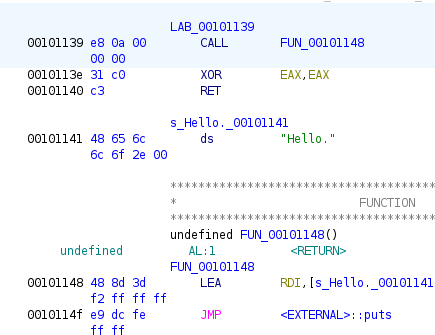
\includegraphics[width=\textwidth]{ghidra-disass-mixed-detail}
\end{frame}


\section{cross-references}
\begin{frame}{cross-references (1)}
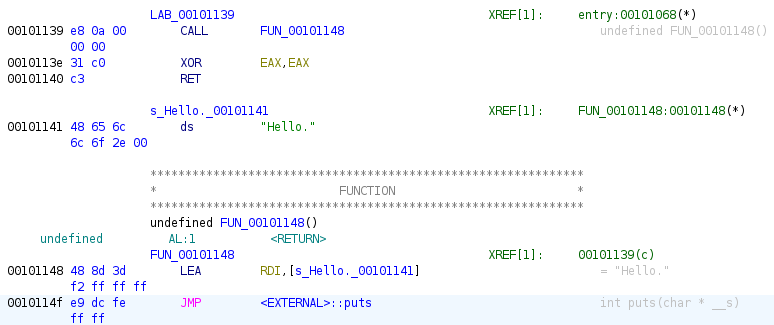
\includegraphics[width=\textwidth]{../re-tools/ghidra-disass-mixed-w-xref}
\end{frame}

\begin{frame}{cross-references idea}
    \begin{itemize}
    \item cross-reference idea:
    \item really useful to know where something is used
    \vspace{.5cm}
    \item do-able `by hand' with objdump and friends, but\ldots
        \begin{itemize}
        \item lots of bookkeeping, searching in text files, etc.
        \end{itemize}
    \end{itemize}
\end{frame}

\begin{frame}{more cross-references}
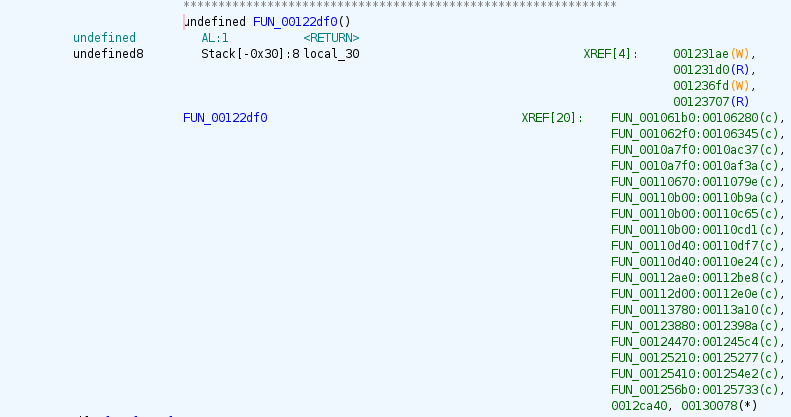
\includegraphics[width=\textwidth]{../re-tools/ghidra-mystery-xref-many}
\end{frame}




\section{high-level overviews}

\subsection{function callers/callees}
\begin{frame}{function callers?}
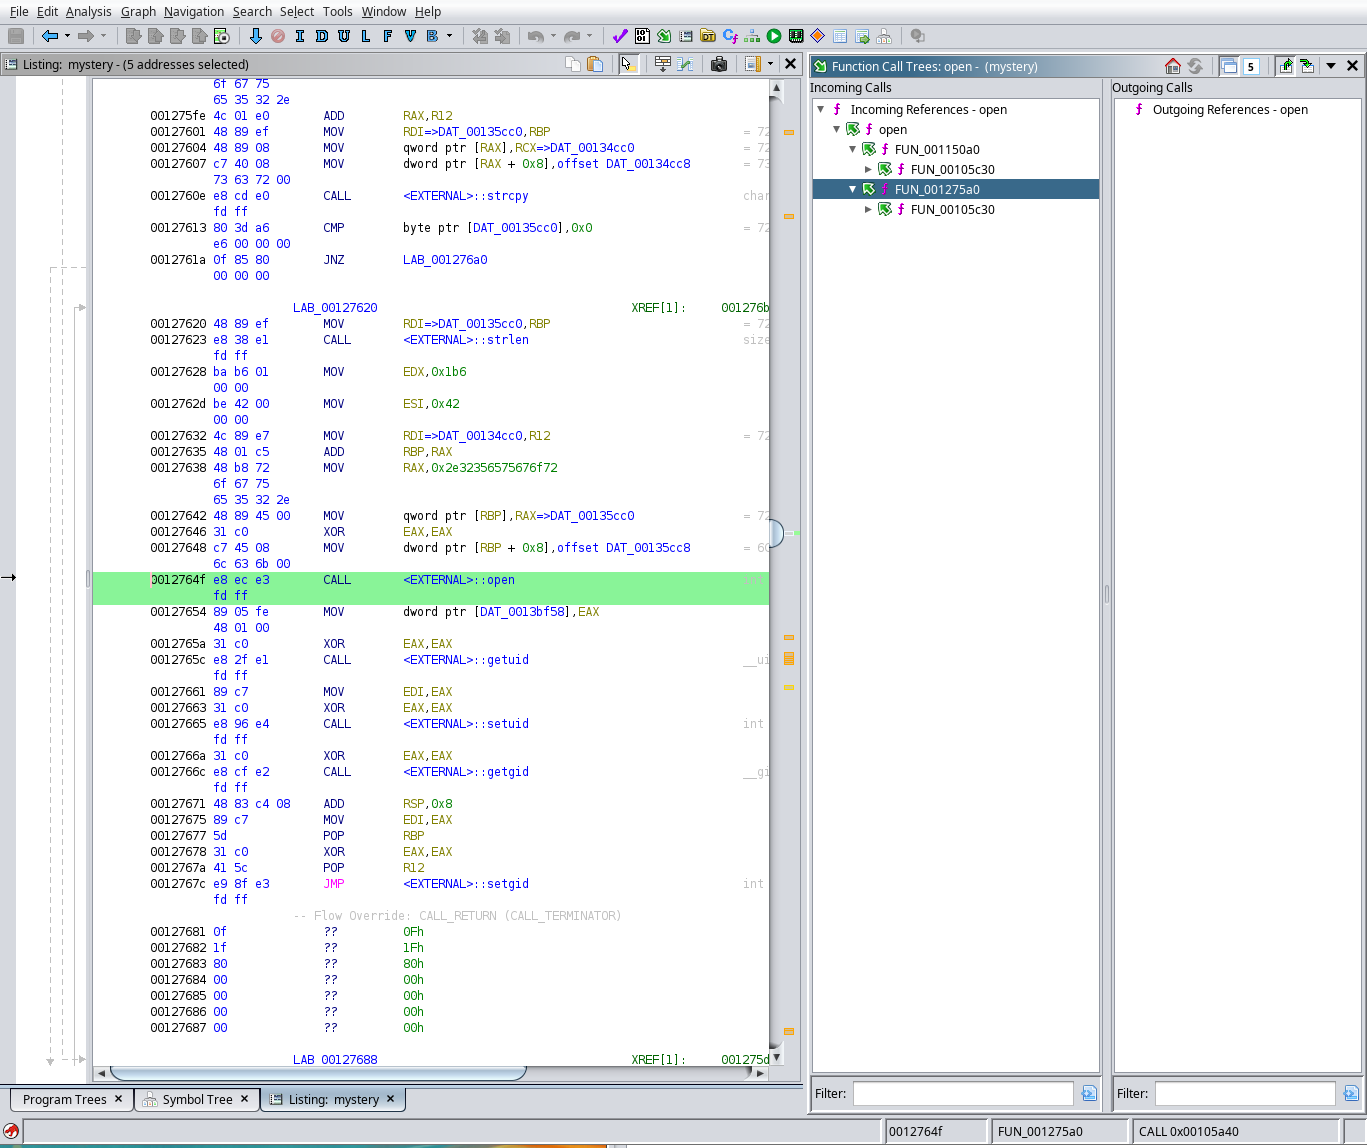
\includegraphics[width=\textwidth]{../re-tools/ghidra-symb-refs-ex}
\end{frame}

\begin{frame}{FUN\_12345678}
    \begin{itemize}
    \item Ghidra names functions without symbols based on address
    \item we can adjust that\ldots
    \end{itemize}
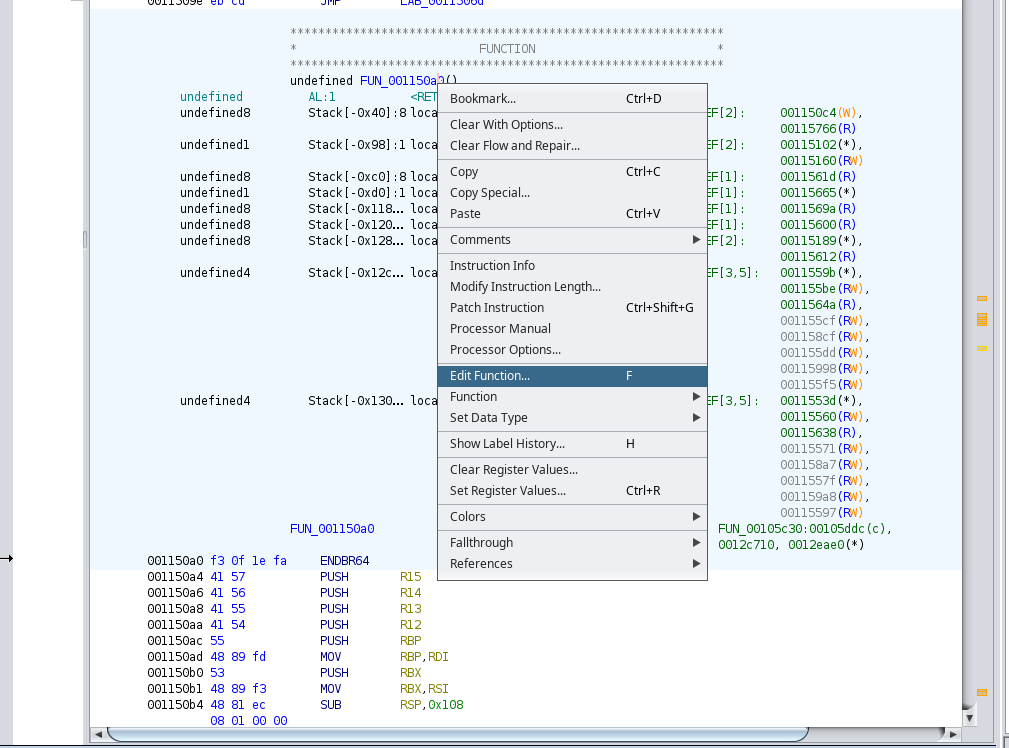
\includegraphics[width=0.45\textwidth]{../re-tools/ghidra-edit-func-cut}
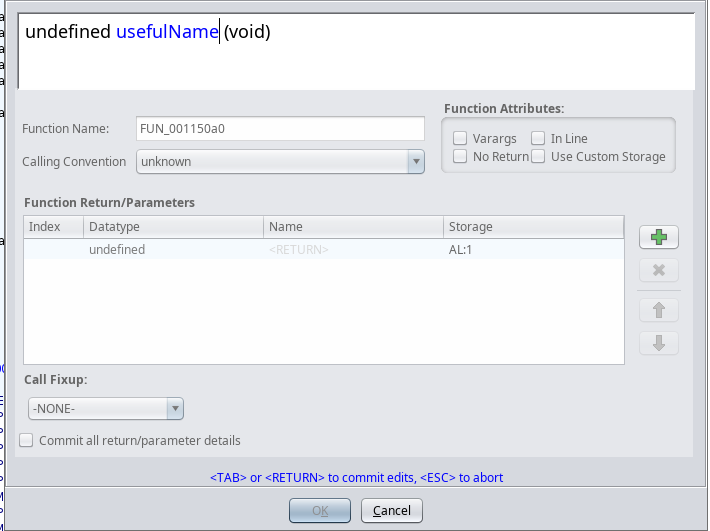
\includegraphics[width=0.45\textwidth]{../re-tools/ghidra-edit-func-dialog}
\end{frame}

 % FIXME: cleanup exercise

\subsection{control flow graphs}
\begin{frame}{}
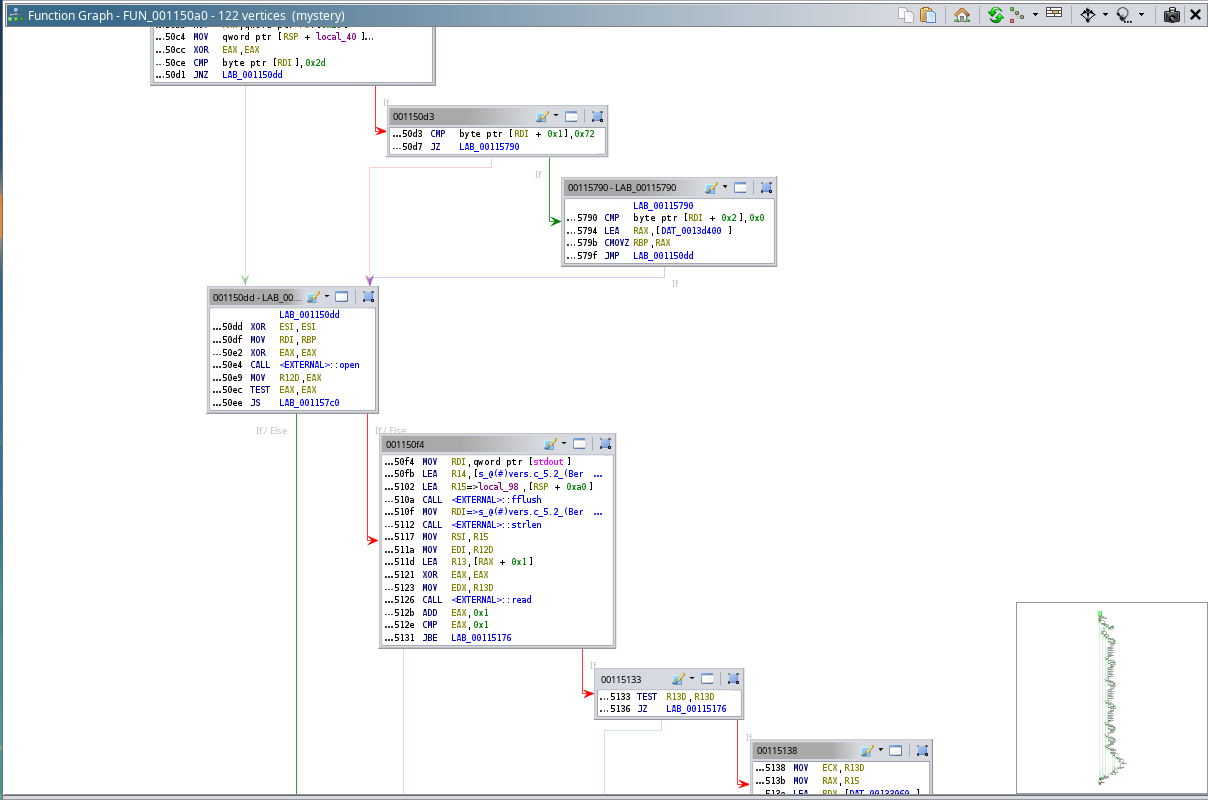
\includegraphics[height=0.95\textheight]{../re-tools/fun-graph-ex}
\end{frame}


\subsection{arrows on the side}
\begin{frame}{}
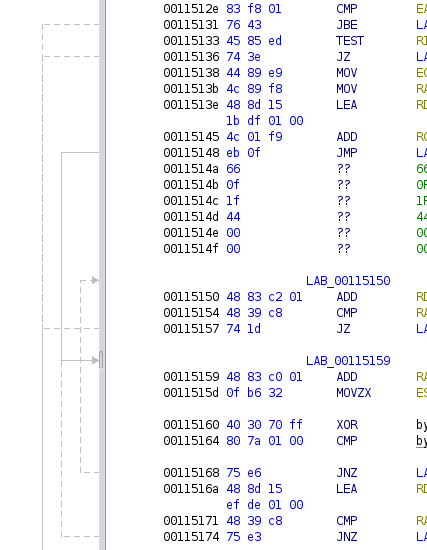
\includegraphics[height=0.9\textheight]{../re-tools/ghidra-side-arrows}
\end{frame}


\section{decompiling}

\subsection{decompiler}
\begin{frame}{decompiler}
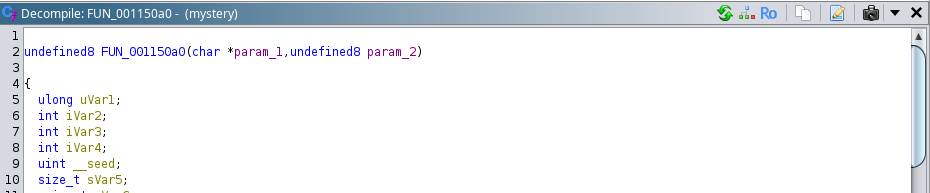
\includegraphics[width=0.9\textwidth]{../re-tools/decomp-top} \\
\ldots  \\
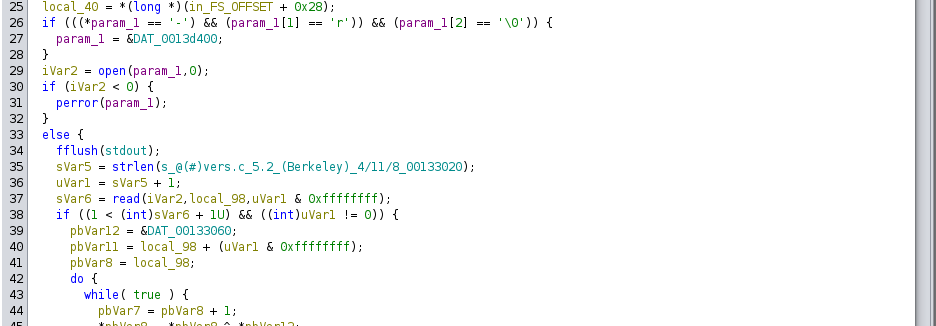
\includegraphics[width=0.9\textwidth]{../re-tools/decomp-rest}
\end{frame}

\begin{frame}{refining decompile (1)}
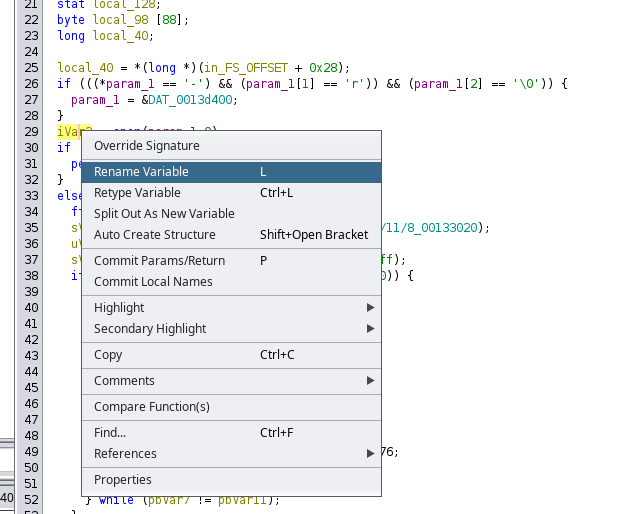
\includegraphics[width=0.9\textwidth]{../re-tools/ghidra-edit-var-decomp}
\end{frame}

\begin{frame}{refining decompile (2)}
    \begin{itemize}
    \item can setup names, types for functions
    \item types can include marking array
        \begin{itemize}
        \item Ghidra doesn't seem great at inferring this all the time
        \end{itemize}
    \vspace{.5cm}
    \item also for local/global variables
        \begin{itemize}
        \item for globals, can right-click in listing view too
        \end{itemize}
    \end{itemize}
\end{frame}



% intermediate representation for main() function in mystery
% decompiled representation
\subsection{Ghidra: intermediate representation}
\begin{frame}{interlude: editing disassembly format}
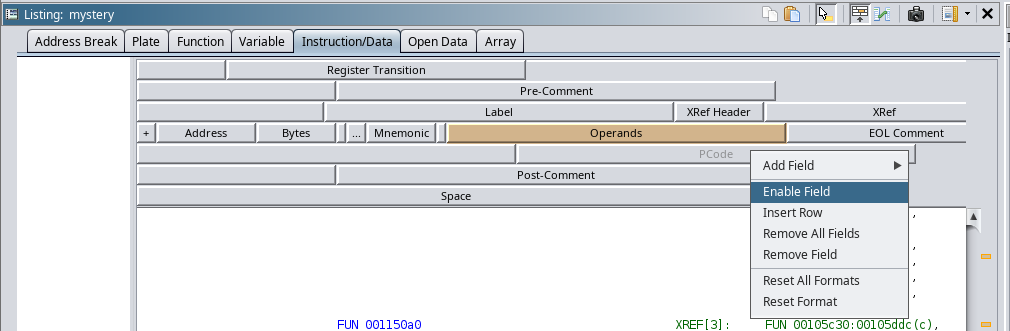
\includegraphics[width=\textwidth]{../re-tools/ghidra-enable-show-pcode}
\end{frame}

\begin{frame}{PCode}
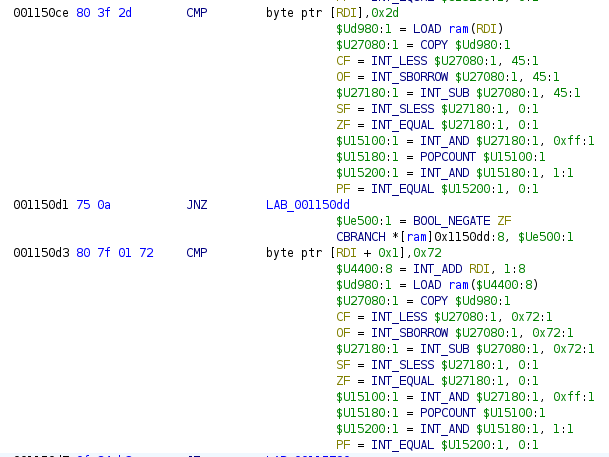
\includegraphics[height=0.9\textheight]{../re-tools/ghidra-pcode-ex}
\end{frame}

\begin{frame}{Intermediate Representations}
\begin{itemize}
\item Ghidra converts instructions to this PCode language
    \begin{itemize}
    \item describes effects of each instruction for other parts of Ghidra
    \item allows `easy' support for ARM, MIPS, \ldots
    \end{itemize}
\item function graph we saw using PCode information, probably
\item decompiler is basically a PCode to C compiler
    \begin{itemize}
    \item does the same kind of optimizations/etc. normal compiler does
    \item different output language
    \end{itemize}
\item Ghidra has `find similar functions' tool that probably uses this
\end{itemize}
\end{frame}




\section{patching things}
\begin{frame}{patch instruction?}
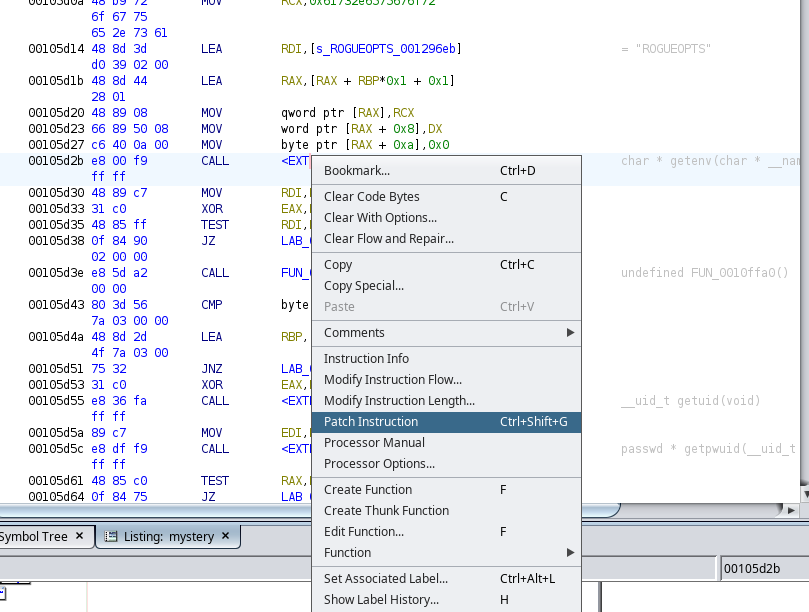
\includegraphics[width=\textwidth]{../re-tools/ghidra-patch-ex}
\end{frame}

\begin{frame}{patch instruction?}
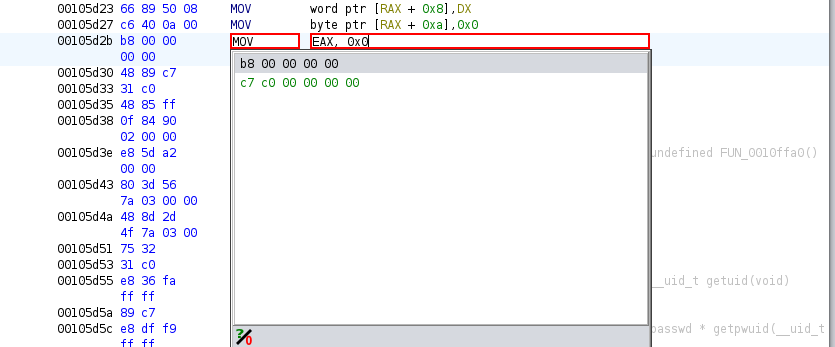
\includegraphics[width=\textwidth]{../re-tools/ghidra-patch-ex2}
\end{frame}

\begin{frame}{why is this useful?}
    \begin{itemize}
    \item can export modified version of binary to test
    \item ghidra has support for debugging or emulating running program
        \begin{itemize}
        \item emulation is another application of PCode representation
        \item debugging requires some work to configure
        \end{itemize}
    \end{itemize}
\end{frame}



\section{on/with debuggers}
\begin{frame}{debuggers / emulators}
    \begin{itemize}
    \item major way to analyzing software --- run it!
    \vspace{.5cm}
    \item possibly using debugger to analyze memory/registers/etc.
    \item possibly in restricted environment
        \begin{itemize}
        \item either limit access to system calls, \textit{or}
        \item run on virtual (okay-to-lose) hardware
        \end{itemize}
    \end{itemize}
\end{frame}

\begin{frame}{selected debugger features}
    \begin{itemize}
    \item watchpoint (GDB/LLDB \texttt{watch})
        \begin{itemize}
        \item breakpoint triggered by variable/expression changing
        \end{itemize}
    \item breakpoints on system calls (GDB \texttt{catch syscall \ldots})
    \item searching memory for strings (GDB \texttt{find}, LLDB \texttt{memory find})
    \item saving `core' files (GDB \texttt{generate-core-file NAME})
        \begin{itemize}
        \item full copy of program's memory, can reload in debugger later
        \end{itemize}
    \item copying memory to/from file (GDB \texttt{dump}/\texttt{append}/\texttt{restore}; LLDB \texttt{memory read}/\texttt{write})
    \item attaching to programs / remote debugging
    \item forcing jump to address/return from function (GDB \texttt{jump}/\texttt{return})
    \end{itemize}
\end{frame}

\begin{frame}{reverse debugging?}
    \begin{itemize}
    \item old idea: `reverse debugging'
    \item in addition to \texttt{step}/\texttt{continue}, \\
        debugger could have \texttt{reverse-step}/\texttt{reverse-continue}
    \item typically implemented by recording `trace' of execution
    \vspace{.5cm}
    \item some implementations (with varyingly middling performance
        \begin{itemize}
        \item \url{https://rr-project.org} for x86-64 Linux (needs sysadmin to set some things)
        \item QEMU for full virtual machines (not just one program)
        \item built-in to GDB, but not maintained/possibly broken with modern systems
        \end{itemize}
    \end{itemize}
\end{frame}

\begin{frame}{Ghidra debugger integration}
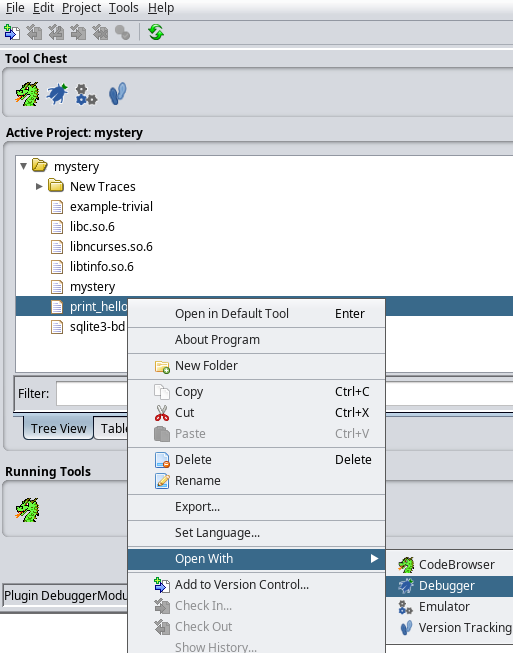
\includegraphics[width=0.35\textwidth]{../re-tools/ghidra-open-debugger.png}
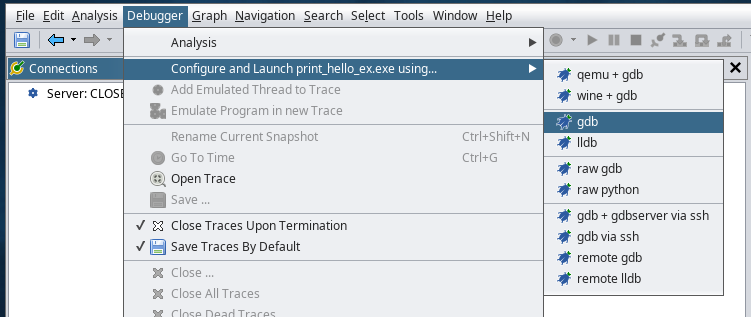
\includegraphics[width=0.55\textwidth]{../re-tools/ghidra-open-debugger2.png}
\end{frame}

\begin{frame}{Ghidra traces}
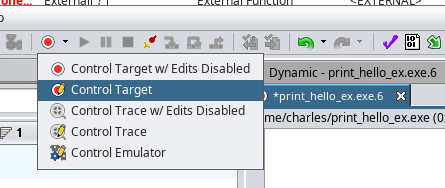
\includegraphics[width=0.3\textwidth]{../re-tools/ghidra-control-target.png}
    \begin{itemize}
    \item Ghidra --- debugging session creates a `trace'
        \begin{itemize}
        \item can be saved to look at later
        \end{itemize}
    \item creates a list of `snapshots' for every time debugger stopped
        \begin{itemize}
        \item snapshots are \textit{incomplete}
        \item need to force read of memory/etc. to have info included in snapshot
        \end{itemize}
    \item can switch between `Control Target' and `Control Trace' modes
        \begin{itemize}
        \item Control Trace --- go back to old snapshots, examine state
        \item Control Target --- control live program in debugger
        \end{itemize}
    \end{itemize}
\end{frame}

\begin{frame}{Ghidra dynamic view}
\begin{tikzpicture}
\node[inner sep=0mm,anchor=north west] (graphic) at (0, 0) {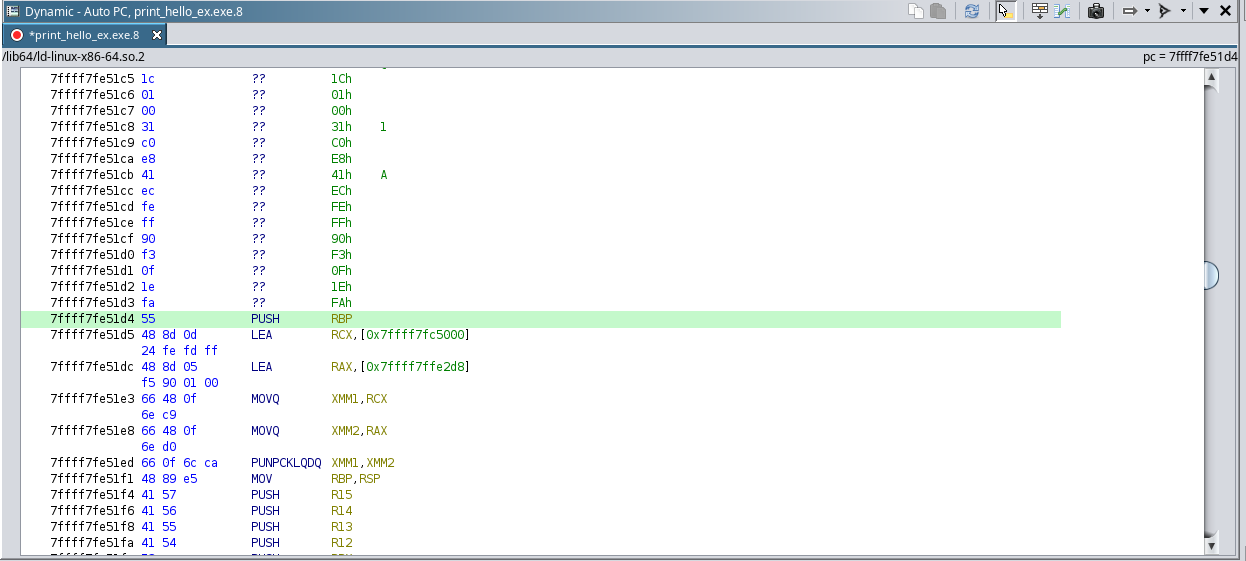
\includegraphics[width=13cm]{ghidra-dynamic}};
%\path[overlay,draw,help lines] (0, 0) grid (14, -8);
\begin{visibleenv}<2>
    \draw[red,thick] (.5, -3.2) rectangle (5, -5.8);
    \node[text=red,anchor=west,align=left] at (5, -5) {
        partial disassembly \\
        (starting from program counter)
    };
    \draw[blue,thick] (.5, -0.8) rectangle (5, -3.2);
    \node[text=blue,anchor=west] at (5, -2) {
        not disassembled by default
    };
\end{visibleenv}
\begin{visibleenv}<3>
    \draw[overlay,violet,thick] (10, 0) rectangle (10.3, -0.2);
    \node[overlay,text=violet,font=\small,anchor=east,align=right] at (10.1, -0.2) {
        reread selected memory
    };
    \draw[overlay,green!60!black,thick] (11.7, 0) rectangle (12.1, -0.2);
    \node[xshift=-1cm,overlay,text=green!60!black,font=\small,anchor=south,align=left] at (11.9, -0.0) {
        select where in \\
        memory to view
    };
\end{visibleenv}
\begin{visibleenv}<4>
    \draw[overlay,red,thick] (11, 0) rectangle (11.3, -0.2);
    \node[overlay,text=red,font=\small,anchor=east,align=right] at (11.3, -0.2) {
        compare memory at different times
    };
\end{visibleenv}
\end{tikzpicture}
\end{frame}

\begin{frame}{Ghidra snapshots/saved traces:}
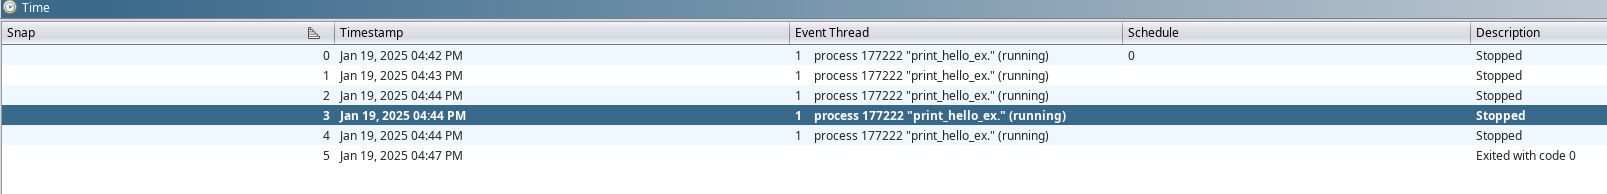
\includegraphics[width=\textwidth]{ghidra-time-trace}
\begin{itemize}
\item automatic partial snapshots whenever pausing debugger
\item can force read of range of memory to make snapshot contain memory image
\end{itemize}
\end{frame}
 % FIXME: screenshots
% FIXME: 
    % remote gdb/lldb
    % taking snapshots and going back to them
    % aside: gdb reverse gdb support

% FIXME: outline for symbolic exec example
    % simple foo(x) { ... } how is X reached?
    % solving for variable
    % then show angr doing this with actual example
    % show automating path in some complex code with angr

    % 
